\documentclass[oneside,final,14pt]{extreport}
\usepackage[utf8]{inputenc}%unix=koi8-r || utf8
\usepackage[russianb,ukrainian]{babel}
\usepackage{vmargin}
\setpapersize{A4}
\setmarginsrb{2 cm}{1.5 cm}{1 cm}{1.5 cm}{0 pt}{0 mm}{0 pt}{13 mm}
\usepackage{indentfirst}
\sloppy %fussy

\usepackage{fancyvrb}
\usepackage{wasysym}
%\usepackage{lscape}
\usepackage{pdflscape}
\usepackage{rotating}

\usepackage{hyperref}

\usepackage{tcolorbox} % code frames

\newenvironment{changemargin}[2]{%
\begin{list}{}{%
\setlength{\topsep}{0pt}%
\setlength{\leftmargin}{#1}%
\setlength{\rightmargin}{#2}%
\setlength{\listparindent}{\parindent}%
\setlength{\itemindent}{\parindent}%
\setlength{\parsep}{\parskip}%
}%
\item[]}{\end{list}}

\usepackage{graphicx}%графика
\graphicspath{{./pic}}
\DeclareGraphicsExtensions{.pdf,.png,.jpg}


\begin{document}

\begin{centering}

\thispagestyle{empty} % нумерация выкл.
\begin{minipage}[t]{16.75cm}
%24

\begin{center}

\includegraphics[scale=0.1]{0}
\end{center}

\vspace{9cm}

\centerline{\Huge  \bfseries Інструкція}
\centerline{\Large \bfseries до емулятора машини Тьюрінга}

\vspace{11,9cm}

\centerline{Булак А.С.}
\vspace{0,2cm}


\end{minipage}

\end{centering}


\pagebreak
	
\tableofcontents
\pagebreak
\setcounter{page}{2}
	
\chapter*{Вступ}
\addcontentsline{toc}{chapter}{Вступ}  
Мета цієї інструкції --- опис можливостей TME, покрокове введення читача у використання емулятора. Відноситься до версії 2.0.0b. Контакти для зв'язку можна знайти у кінці інструкції.

\bigskip

Інструкція складається з декількох частин, кожна з яких об'єднує близькі за темою глави:

Частина нуль коротко описує варіати поставки емулятора, можливі додаткові ресурси.

Перша частина описує мову емулятора, загальну структуру цієї 
формальної~
\footnote{Важливий термін, до якого я буду звертатися ще багато разів. Уникаючи громіздких математичних формулювань, можна сказати так: Формальна мова --- це множина слів (у нашому випадку --- рядків), що сформовані з множини алфавіту, за множиною правил.}
мови, її обмеження, пояснюється логіка її проектування. З метою навчити користувача вирішувати виникаючі проблеми, коротко описується внутрішній устрій емулятора.

Друга частина розповідає про графічну версію програми. Наводяться описи інтерфейсу, розповідається про загальні підходи до його проектування, ексклюзивні можливості програми. 

Третя частина описує ??? % парадигми

Також в інструкції є додатки, що містять приклади програм, додаткові матеріали, мої контакти.

\bigskip

\bigskip 

Необхідною є перша частина. Користувачів графічного додатка може зацікавити частина два, користувачів консольного --- нульова. Корисно переглянути додатки.

Досвід роботи з різними інтегрованими середовищами розробки (IDE) значно полегшить розуміння викладеного, як і знання мов C, будь-якого з сімейства Assembler, та текстового редактора Vim.

\bigskip

\bigskip

Якщо сподобається емулятор --- можете залишити зірочку у моєму  \href{https://github.com/Kaifolog/TME}{репозиторії}.

\setcounter{chapter}{-1}

\chapter{Дистрибуція}

Я не намагався здавати індивідуальне завдання з консолі, тому попереджую,
\marginpar[]{\Huge \bfseries !} 
 що викладачі можуть не прийняти його у вас. А можуть і прийняти, перепитайте.
 
\vspace{0.4 cm}
 
 Консольна версія програми розповсюджується у вигляді вихідних текстів мовою C++. Проект використовує систему збирання CMake.
 Звісно, CMake не є самостійною, отже, перелічимо повний список необхідних утиліт для збирання консольної версії:
  
 \begin{enumerate} 
  \item C і С++ компілятори. Я використовую GNU gcc / MinGW / Clang.
  \item  GNU make / mingw32-make / Clang make. (Ці програми є у стандартній поставці компіляторів з п.1)
  \item CMake.
\end{enumerate}
  
Важливо знати: для вибору між консольною та графічною версією використовується CMake флаг \fbox{IS\_GUI}. За замовчуванням його значення дорівнює \fbox{FALSE}, тобто за замовчуванням збирається консольна версія.

\section{Збирання консольного додатку}
Перебуваючи у корні проекта треба, на догоду чистоті та акуратності, створити папку build, згенерувати make файли з cmake, а потім запустити збирання за допомогою make.
Зробимо це:
\begin{verbatim}
Windows:
(для MinGW, інші toolchains - інший аргумент типу makefiles 
і виклик make, детальніше у документації CMake про -G флаг)
\end{verbatim}
\begin{tcolorbox}
\begin{verbatim}
mkdir build && cd build
cmake .. -G "MinGW Makefiles"
mingw32-make
\end{verbatim}
\end{tcolorbox}

Треба згадати про WSL і проблеми, які він може створити. Через конфлікти кодувань тексту і багато іншого я не рекомендую використовувати емулятор на WSL. Ця зв'язка працює нестабільно.

\begin{verbatim}
Linux/WSL/MacOS:
\end{verbatim}
\begin{tcolorbox}
\begin{verbatim}
mkdir build && cd build && cmake .. && make
\end{verbatim}
\end{tcolorbox}

Це й же шлях компіляції буде працювати для MacOS'ісвського clang toolchain з його власним make.

Виконуваний файл треба шукати у піддиректорії build/src/emulator.

\section{Збирання графічного додатку}

Для збирання графічної версії до перелічених вище програм додається наявність на машині qt5 framework у його поставці у вигляді dll's.

Отже, треба встановити qt5 та перебуваючи у корні проекта зібрати додаток:


\subsection{Windows}

Нажаль у windows архітектурно не передбачено системних директорій для бібліотек, як і не передбачена проста робота з ними. Отже, треба встановити з офіційного сайта qt 5 версію бібліотеки у якусь папку, та запам'ятати її назву. У лістингу вона буде названа \$path\$
\begin{tcolorbox}
\begin{verbatim}
mkdir build && cd build

cmake .. -G "MinGW Makefiles"
-DCMAKE_PREFIX_PATH="$path$/$qt version$/$qt compiler copy$" 
-DIS_GUI=True

mingw32-make
\end{verbatim}
\end{tcolorbox}

Про запуск qt додатків з динамічними залежностіми є багато в інтернеті. Можна покласти exe файл у директорію, що вказана у флазі DCMAKE\_PREFIX\_PATH, або скористатися тим набором бібліотек, які використовує реліз з мого github.

Шукати виконуємий файл треба у піддиректорії build/src.

\subsection{Linux}

Робота з qt на Linux набагато приємніша ніж на Windows. Отже, скористуємося apt та наявністю /lib директорії.

\begin{tcolorbox}
\begin{verbatim}
sudo apt update
sudo apt install qt5-default
mkdir build && cd build
mkdir build && cd build && cmake .. -DIS_GUI=True && make
\end{verbatim}
\end{tcolorbox}

Шукати виконуємий файл треба у піддиректорії build/src.

Linux сам у runtime знайде та підключе необхідні бібліотеки.

\subsection{MacOS}

Необхідна наявність \textbf{\href{https://brew.sh}{brew}}.

Робота з qt на MacOS приємніша ніж на Windows. Отже, скористуємося brew та наявністю у brew директорії з бібліотеками.

\begin{tcolorbox}
\begin{verbatim}
brew install qt5
brew --cellar qt@5
\end{verbatim}
\end{tcolorbox}
У відповідь на другу команду, після успішної установки qt5, буде виведено абсолютний шлях до папки qt бібліотек.

Треба перейти по ньому (замість мого треба вставити свій шлях):

\begin{tcolorbox}
\begin{verbatim}
~:cd /opt/homebrew/Cellar/qt@5
~:ls
  5.15.2_1
~:cd 5.15.2_1
~:pwd
  /opt/homebrew/Cellar/qt@5/5.15.2_1
\end{verbatim}
\end{tcolorbox}

Отриманий шлях треба передати CMake аргументом DCMAKE\_PREFIX\_PATH (замість \$).

\begin{tcolorbox}
\begin{verbatim}
mkdir -p build && cd build
cmake .. -DIS_GUI=True -DCMAKE_PREFIX_PATH="$" && make
\end{verbatim}
\end{tcolorbox}

Шукати виконуємий файл треба у піддиректорії build/src.

MacOS сама у runtime знайде та підключе необхідні бібліотеки.

\section{Опис інтерфейсу консольного додатку}
Після оформлення програми згідно правилам попередньої частини, треба зберегти файл з текстом програми та викликати емулятор з відповідними аргументами. Ось пояснення до їх використання:
\bigskip
		
"<Визначаючим"> аргументом є найперший з них.
		
Якщо першого аргументу взагалі немає, тобто пишемо,
\begin{tcolorbox}
\begin{verbatim}
Windows:
start TME.exe

UNIX-like:
./TME
\end{verbatim}
\end{tcolorbox}
то програма виведе інформацію про свою версію та невелику інструкцію англійською.
\\	
Якщо,
\begin{tcolorbox}
\begin{verbatim}
Windows:
start TME.exe -v

UNIX-like:
./TME -v
\end{verbatim}
\end{tcolorbox}
ми можемо дізнатися про версію емулятора та побачити лого з обкладинки.

Якщо перший аргумент це шлях до файлу, ми маємо право вказати "<непозиційні аргументи">, список яких наведено нижче. Шлях до файла без непозиційних аргументів рівносильний "<./TME ../example.txt -g -a -e">.
		
		
\begin{tcolorbox}	
\begin{verbatim}
	Windows:
	TME.exe $path to programm$/programm.tme $KEYS$

	UNIX-like:
	./TME $path to programm$/programm.tme $KEYS$
\end{verbatim}
\end{tcolorbox}
		

\$KEYS\$ $\subset$ \{-g, -a, -e, -l, -d\}
			
		
		Де:
		
		
\begin{tabular}{ l l }
	-g & генерація бд команд і інших тимчасових файлів \\
	-a & аналіз команд, що підказує, можливо, \\
	   & потрібні команди та вказує на фатальні помилки \\
	-e & запускає емулятор, після емуляції буде створений\\
	   &  файл $*\_out.txt$ , з вихідним рядком \\
	-l & замінює всі входження lambda на " " пробіли\\
	-d & debugger\\ 
\end{tabular}

Сподіваюся про логування пояснювати не треба. Записи можна подивитися у файлі "<name\_log.txt">, де name це назва вхідного файла.

\section{Консольний debugger}
Після розставлення точок зупину, можна запустити дебагер командою
\begin{tcolorbox}	
\begin{verbatim}
	Windows:
	TME.exe $path to programm$/programm.tme -d

	UNIX-like:
	./TME $path to programm$/programm.tme -d
\end{verbatim}
\end{tcolorbox}

Після генерації і аналізу запуститься дебагер, та буде виконувати програму у по-рядковому режимі з першого ж рядка.
Для того щоб виконувати програму по рядку, треба натискати "<Enter">. Щоб перейти до наступної точки зупинки --- введіть непорожню послідовність символів, і натисніть "<Enter">.

{\bfseries Спробуйте зараз!}

У випадку помилкі між точками зупину, программа сама зупиниться та покаже вміст машини та її параметри.

\chapter{Мовне питання}
У таких емуляторів існує кілька видів інтерфейсів. Два основні види --- текстовий інтерфейс та інтерфейс з використанням полів вводу --- так званих форм. Через необхідність працювати з емулятором на різних операційних системах був обраний перший варіант. Графічні інтерфейси пишуться та збираються доволі тяжко і рідко бувають "<реально"> кроссплатформними.
\section{Шлях}
Щоб розуміти якесь рішення, треба розуміти його природу, причини, з яких воно склалося. Ось і ми у цій брошурі підемо шляхом хоробрих архітекторів: будемо стикатися з проблемами та вирішувати їх, зазвичай, найпростішим шляхом.

На початку другого семестру ви повинні були познайомитися з машиною Тьюрінга. На жаль, на відміну від теорії, реальність не можна придумати; у моєму другому семестрі існувало декілька неідеальних емулятори, кожен з яких мене чимось не влаштовував. 

Оніщенко
\footnote{Я поважаю його та його працю, але я змушений відмовляти вас від використання цього емулятора. Програма має "<витоки пам'яті"> та помилки часу виконання, що викликає різні емоції при його "<зхлопуванні"> без збереження вашої кількагодинної праці.}
 "<лається"> на пробіли, таблиці виглядають громісткими (чесно кажучі, я навіть не намагався в них писати --- страшно), і жоден з них не працював на UNIX-системах\footnote{Загальноприйнятий термін. У вузькому сенсі Linux, MacOS.}.

Існує ще декілька моїх вимог, які жоден емулятор не міг задовольнити. По-перше, необхідні коментарі. Через те, що наша формальна мова є регулярною  --- рядки мало відрізняються один від одного, і вже за 20 рядків, програма стає темним та страшним лісом. Треба віддати належне табличним емуляторам, вони це вміють, але не у тій формі, яку я хочу.
Друга вимога --- хороший, приємний дебагер, схожий на один з тих, що є в популярних IDE
\footnote{IDE --- інтегрована середа розробки. VS, Eclips, PyCharm --- такі приклади.}
. Третя і остання вимога --- зрозумілий формат зберігання програми. Це вирішує декілька серйозних проблем водночас: легко зберігати та передавати
\footnote{Насправді, емулятор побудований навколо ідеї, що жодна робота не повинна пропасти. Все повинно зберігатися у постійній пам'яті.}
, легко правити у будь-якому редакторі, якщо вам не подобається мій.

\section{Структура команди}

Мені сподобалася форма команди з Оніщенка, вона має наступний вигляд:

\begin{verbatim}
	state1, word1 -> state2, word2, direction
\end{verbatim}

Всі state1, state2 мають складатися тільки з латинських літер верхнього та нижнього регістру, цифр та символу нижнього підкреслення "<$\_$">.
		
У word1, word2 також допустимі латинські літери верхнього та нижнього регистру, але тільки такі спецсимволи: $+,-,/,*,=,:,\hat{•},\#,!,?,\&,>,<,\%,\_$\\ (без коми!). 
		
Не мають обмежень щодо довжини (не гарантую >256 символів), не мають обмежень щодо пробілів.
\\
"<direction">  може мати тільки такі значення $\{R,r;L,l;S,s\}$.

Отже:
		
\vspace{0.2cm}
		
\begin{tabular}{ | l | l | }
	\hline
	"<Тип сутності"> & Множина допустимих символів \\ \hline
	state1, state2 & латинські літери верхнього та нижнього регистру,\\
	& числа та символ нижнього підкреслення "<\_">. \\
	\hline
	word1, word2 & латинські літери верхнього та нижнього регистру,\\ 
	& числа, спецсимволи: $+,-,/,*,=,:,\hat{},\#,!,?,\&,>,<,\%$.  \\
	\hline
	direction & $R,r;L,l;S,s$ \\
	\hline
\end{tabular}

\section{Вхідний рядок}
Згідно з теорією, машина має нескінченну у дві сторони стрічку, розділену на клітинки. Вважаючи всі клітинки, окрім визначених нами, порожніми, звузимо нашу задачу до скінченного рядка.

Вважатимемо, що я вирішив розділяти клітинки стрічки пробілом "< ">, бо це найбільша клавіша на клавіатурі. 

Але залишається ще два питання: пустий символ, бо пробіл вже зайнятий, та текстове подання курсора. Пустим символом я обрав "<lambda">, маленькою латинецею; курсором буде символ "<|">, з двох сторін від обраної клітинки. Цей символ зазвичай знаходиться над клавішею Enter (натисніть Shift+"<\textbackslash{}">).

Наведу приклад вхідного рядка:
\begin{verbatim}
	|1| 0 lambda 1 1 1 0 *
\end{verbatim}

{\bfseries Для отримання пустих клітинок з боків від введених даних не потрібно писати їх руками. При спробі здвинути курсор на поки неіснуючі клітинки програма сама створить їх пустими.}

\section{Структура програми}
Зважаючи на завдання з глави 1.1, метою є створення мови, яка б мала зручне текстове подання.

Так як машина Тьюрінга має два різні по своїй сутності типи вхідних даних (тобто множину команд та вхідний рядок), треба знайти спосіб вмістити все в один текстовий файл заради  "<легкості зберігання та передачі">.

На порятунок приходить секційний стиль мов асемблера.
Асемблери теж зберігають все в одному файлі, роблячи це в окремих секціях, для чого використовують директиви
\footnote{Деякі читачі можуть згадати ще третю директиву визначення секції, але вона нам ні до чого.}
:
\begin{verbatim}
	section .data
	section .text
\end{verbatim}
Пристосуємо їх до нашої формальної мови. Відповідно до назви, секція .data буде зберігати в собі вхідні дані, тоді як .text --- текст програми, тобто множину команд.

{\bfseries Важливо зауважити, що під час аналізу тексту програми серед .data обирається остання, а всі .text зливаються в одну. Кінцем секції вважається початок іншої або кінець файла.}

Машина має два особливих стани --- початку та кінця програми. Їх ми назвемо "<start"> та "<end"> відповідно.

Приклад простої програми, що ставить на стрічку одну одиницю:
\begin{verbatim}
	section .data
	|lambda|
	section .text
	start, lambda -> end, 1, s
\end{verbatim}

\section{Макроси та де вони макро-}
Всі читачі, які знайомі з мовою С
\footnote{С++ це дещо інше, макропідстановки грають меншу роль. Я не знаю. Я чув.}
, знають, яку велику роль грають макроси у написанні програми.

Макроси нашої мови мають той же механізм роботи, що макропідстановки мови С, тобто заміняють один шматок тексту на інший.
		
Продемонструємо синтаксис макроса:
		
\begin{verbatim}
	#define >> ->
\end{verbatim}
		
Аргументи можуть мати довільну довжину. Макрос завжди починається з директиви {\ttfamily \#define}, між директивою та її двома аргументами має бути по одному пробілу. Макросам все-одно що в них, вони сприймають будь-які символи. Після першого пробілу, в тексті частини що "<підставляється"> (у другому аргументі), можуть будти пропуски, але я не рекомендую так робити.

{\bfseries		
Область дії макросів - лише section .text. 

Макроси нашої формальної мови не здібні до "<зациклювання">, замінюючи один одного. При роботі емулятора створюється таблиця в оперативній пам'яті, кожен рядок якої --- макропідстановка. Макропроцесор перебирає всі рядки таблиці один раз, не зважаючи на успішність підстановки. Звідси ще два правила --- макроси працюють тільки після їх появи в таблиці, тобто тільки нижче рядка їх оголошення; макроси підставляються у послідовності їх оголошення.
}

Продемонструємо роботу макросів на прикладі програми xor:	
\begin{verbatim}
	#define :: _ZnU11_
	#define >> ->

	section .data
	|1| 0

	section .text
	start,0->start,0,r	;проходимо вправо від двох бітів.
	start,1->start,1,r	;
	start,lambda->xor::start,lambda,s

	;xor::start
	xor::start, lambda >> xor::transit1, lambda, l 
	xor::transit1, 0 >> xor::nub1_0, lambda, l
	xor::transit1, 1 >> xor::nub1_1, lambda, l
	xor::nub1_0, 0 >> xor::ret, 0, r
	xor::nub1_0, 1 >> xor::ret, 1, r
	xor::nub1_1, 0 >> xor::ret, 1, r
	xor::nub1_1, 1 >> xor::ret, 0, r 
	;xor::ret

	xor::ret, lambda -> end, lambda, s
\end{verbatim}
У прикладі макроси заміняють стандартний оператор переходу "<->"> на "<>{}>">, та дають змогу використати "<::"> подібно до мови С++.
		
Я пропоную використовувати нечитаємі комбінації літер та чисел для макросів, які ви використовуєте як оператор області видимості.
		
Таким чином, макроси та структура нашої програми дозволяє нам писати окремі модулі-секції з обумовленими точками входу та виходу, своїми просторами імен.
\section{Коментарі}

Як ви могли помітити у попередній главі, мова має коментарі. Вони мають однорядковий синтаксис та починаються з символу "<;">, {\bfseries працюють у секції коду}.

Згідно з ассемблерними традиціями, такі коментарі ставлять через табуляцію від рядка програми. Зазвичай, коментарі вирівнюють до одного рівня, ось приклад:

\begin{Verbatim}
	section .text
	start, lambda ->  world, Hello, r	  ; printing Hello
	world, lambda -> name, World, r	    ; printing World
	name, lambda -> exclamation, %username%, r ; printing username
	exclamation, lambda -> end, !<3, r         ; printing exclamation
	                                           ; sign and ending
\end{Verbatim}
\section{Breakpoints}
Всі дебагери, що я бачив у таких емуляторах, не використовували точки зупину, тому я був вимушений вигадати їм текстовий аналог.

Ось що вийшло:

\begin{Verbatim}
	section .text
	start, lambda ->  world, Hello, r	  
	world, lambda -> name, World, r	    ;#d
\end{Verbatim}
"<;\#d"> --- точка зупинки. 

Я не рекомендую залишати коментарі після точок зупинки, хоча така можливість і існує.
\section{А скринька просто відкривалась...}
\label{chap:emulator:func}
Як і у випадку з компіляцією мови С, але з трохи інших причин, користувач повинен мати уявлення про внутрішні процеси, що відбуваються під час емуляції.

\begin{figure}
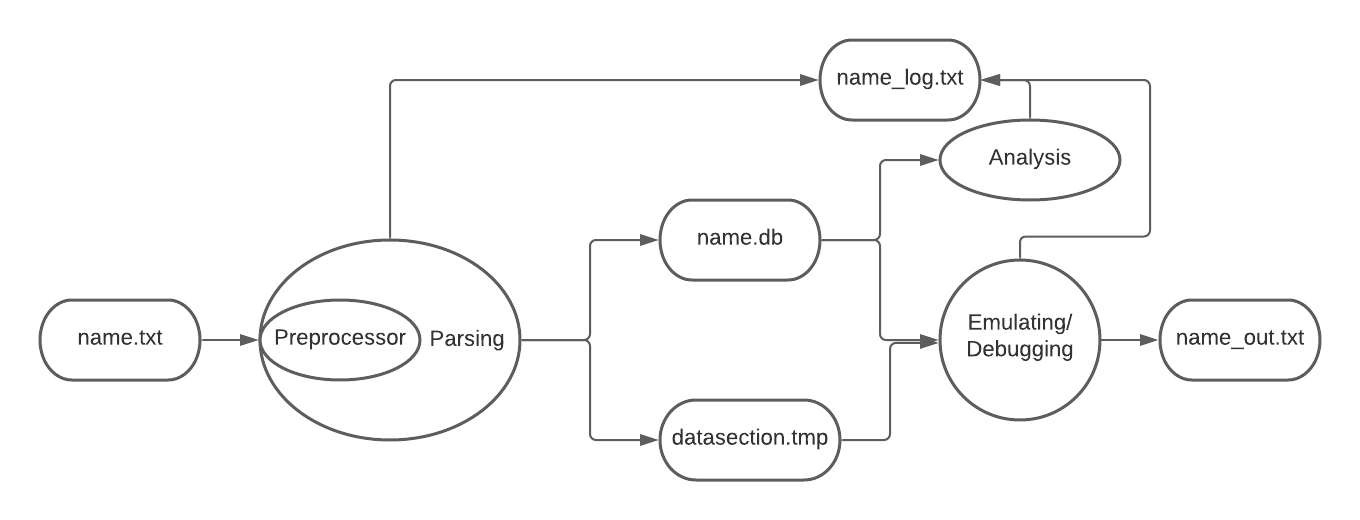
\includegraphics[scale=0.8]{2}
\caption{Схематичне зображення "<тракту"> емулятора.}
\end{figure}

Роботу нашого емулятора можна розкласти на три окремі режими, що можуть комбінуватися різним чином (Рис 1.1).

Першим і найважливішим є режим обробки вхідного тексту (Parsing). Після отримання вхідного коду, емулятор відділяє секцію даних у файл "<datasection.tmp">, який завжди лежить у директорії виконуваного файла та є тимчасовим, файл перезаписується при новій обробці вхідного тексту. Одразу після цього емулятор записує множину команд у таблицю спеціального виду, яку зберігає у файл з розширенням "<.db"> (db від англ. database --- база даних). Перед складанням таблиці команд, підставляються всі макроси.

Аналіз є необов'язковим етапом. На вхід він отримує таблицю команд, яку згенерував режим "<Parsing">. Взагалі, режим задумувався як статичний аналізатор користувацької програми, але сьогоднішні його можливості найскромніші, єдине його прикладне застосування, на мій погляд, це перевірка наявності станів початку та закінчення. Механізм дії елементарний: перевірка наявності всіх станів для всього зовнішнього алфавіту, і навпаки; перевірка наявності початкового та кінцевого станів.

Емуляція і відладка, по своїй суті, відрізняються тільки способом виконання одних і тих же дій. У цьому режимі створюється об'єкт машини, у який загружається вхідна стрічка, яка після цього обробляється на основі таблиці команд. Вихідна стрічка записується у файл, назва якого закінчується на "<\_out.txt">; звісно, тільки у випадку успішного виконання.

Про роль файлу "<\_log.txt"> я розповім трохи пізніше.

\chapter{Запуск, графічний додаток}
\section{Що треба знати, щоб уникнути помилок?}
GUI
\footnote{GUI - (Graphical User Interface) графічний інтерфейс користувача.}
 додатку створений на основі фреймворка Qt.

Додаток потребує динамічні бібліотеки (.dll), які він "<підгружає"> у процесі виконання. 
Бібліотеки можна лінкувати статично, але для цього треба прикласти певні зусилля. Якщо ви вважаєте це необхідним --- напишить мені листа на пошту.

\textbf{Windows:}

Для роботи програми необхідно ніяк не змінювати структуру папки з релізного архіву, в якому вона поставляється.

Я рекомендую створити ярлик до .exe файла та покласти його у зручне для вас місце.

\textbf{Linux:}

Для запуску релізу необхідно \textbf{надати програмі права на виконання} та встановити qt5 бібліотеки.
\begin{tcolorbox}	
\begin{verbatim}
sudo apt install qt5-default
./TME
\end{verbatim}
\end{tcolorbox}

\textbf{MacOS:}

Для запуску релізу необхідно \textbf{надати програмі права на виконання} та встановити \textbf{\href{https://brew.sh}{brew}} та qt5 бібліотеки.
\begin{tcolorbox}	
\begin{verbatim}
brew install qt5
./TME
\end{verbatim}
\end{tcolorbox}
		
За замовчуванням використовується темна тема Google Material Dark, що може бути незручним при використанні, наприклад, під палким Кримським сонцем. Щоб відключити тему, треба знайти в папці проекта файл MaterialDark.qss та змінити його назву, наприклад: "<MaterialDark1.qss">, перезапустити програму. Після цього штатно застосується біла тема.

\section{Загальні підходи до проектування GUI.}
Будь-яка людська робота важлива з великої кількості причин. Працюючи на емуляторі Оніщенка, я декілька разів втрачав свої програми. Отже, треба від цього захиститися.
		
Заради збереження нашого часу та нервів, при роботі з графічним інтерфейсом ми обов'язково повинні спочатку відкрити чи створити файл. Це запобігає втраті коду при виникненні непередбачених помилок у емуляторі.

Всі сучасні операційні системи мають "<системний журнал">, туди записується кожен рух користувацьких програм та всі події, які відносяться до операційної системи. Це "<чтиво"> має суто прикладну цінність: коли щось йде не так, можна "<відмотати"> час назад та зрозуміти що призвело до катастрофи. Цей прийом називають логуванням (англ. logging), ми будемо його використовувати.
\section{Опис інтерфейсу}
Скріншот програми є на сторінці \,\pageref{screenshot}.
\medskip

Майже всі елементи інтерфейсу підписані, сподіваюся ви зорієнтуєтеся по тексту.

Почнемо з найбільшого елемента --- поля редагування тексту. Нажаль, Qt не має простих інструментів додавання колонки нумерації рядків. Звісно, залишатися без нумерації --- це залишатися без засобів відладки програми. Результатом цих обставин стала Vim-style нумерація, яку можна побачити справа знизу, під панеллю логів. Поле показує номер рядка на якому стоїть курсор. Сама панель логів не потребує представлення.

Перейдемо до двох довгих смуг зверху вікна ---  "<Input data line"> та "<Output/Debug line">, до чекбоксів
\footnote{(від англ. check box) флагова кнопка, галочка.}
поряд. "<Output/Debug line"> --- поле у якому показуються результати роботи або поточний стан стрічки машини під час процесу відладки. Як на мене, "<lambda"> у великому вихідному рядку іноді дезорієнтує, тому я створив  чекбокс "<lambda as space">, що замінює всі входження "<lambda"> на "< "> у "<Output/Debug line">. Чекбокс починає працювати при наступному виводі даних.

Поясню про "<Input data line">, ідея цього рядка --- тримати вхідну стрічку перед очима користувача та візуально відокремлювати від секції тексту. Це поле нерозривне у своєму використанні з чекбоксом "<.data to data line">. При натисканні на вимкнений чекбокс, емулятор порівнює перший рядок файла з рядком "<section .data">, якщо вони збігаються --- секція "<виймається">, її вміст записується у "<Input data line">. При відтисканні кнопки відбувається зворотній ефект, тобто секція дописується зверху файла, навіть коли вона порожня. Спробуйте, інакше не зрозумієте!

Нижній лівий кут має ідентифікатор стану файлу ("<Saved">, "<Changed">), та показує n символів з кінця абсолютного шляху до файла.

Про режими роботи емулятора я згадував у главі
\ref{chap:emulator:func}, кнопки зправа зверху --- це втілення режимів "<у металі"> з однією надбудовою: з'явилася кнопка "<Quick start">, Quick start=Parsing+Emulation.

Верхнє меню складається з декількох вкладок, вкладка "<File"> виконана стандартно для текстового редактора, інші носять інформаційний характер.

\begin{changemargin}{-10,3cm}{1,1cm}
\begin{landscape}
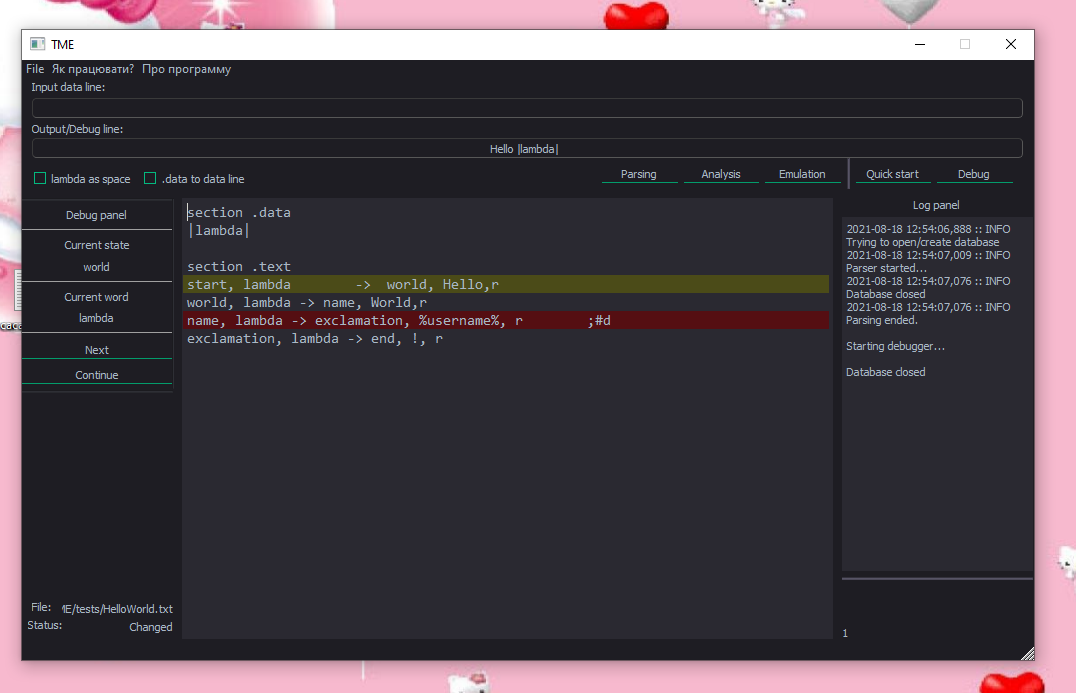
\includegraphics[scale=0.94]{1}
\label{screenshot}
\end{landscape}
\end{changemargin}

\newpage
\section{Debugger}
Скріншот програми є на сторінці \,\pageref{screenshot}.
\medskip

Суть роботи відладника в тому, щоб дати користувачу виконувати покроково проблемні відрізки програми. Для цього використуються breakpoints, вони ж "<точки зупину">. Залишаючи їх, користувач просить дебагер зупинитися на конкретному моменті виконання та чекати подальших вказівок. Крім того, дебагер дозволяє у будь який момент часу дізнатися параметри машини та подивитися її стрічку.

Після натискання на кнопку "<Debug">, дебагер зупиняється на першому рядку та чекає наших інструкцій. Debug panel має дві кнопки "<Next"> та "<Continue">. Перша робить один крок дебагера, інша змушує відладник йти до наступної точки зупину, помилки, кінця програми. У всіх трьох випадках він поводиться однаково --- показує в панелі свої останні параметри.
Звісно, кнопки "<Next"> та "<Continue"> працюють тільки у режимі дебагу.

У режимі дебагера точки зупину підсвічуються червоним, поточний рядок --- жовтим.

Знову ж, краще спробувати.
\section{Гарячі клавіші}
\label{sec:hotkeys}
\begin{tabular}{| l | l |}
	\hline
	Комбінація & Дія \\
	\hline
	Ctrl+S & Зберігає відкритий файл. \\
	\hline
	Ctrl+O & Ініціалізує відкриття файла. \\
	\hline
	Ctrl+N & Ініціалізує створення файла. \\
	\hline
	Ctrl+Shift+X & Quick start. \\
	\hline
	Ctrl+Tab & Аналізує рядок, на якому стоїть курсор \\
	 		 &  та доповнює його до форми "$,->,,\setminus$n".\\
			 & Аналог "<Tab"> з емулятора Дікарева.\\
	\hline
	F5 & Робить 1 ітерацію у debug режимі.\\
	\hline
	Ctrl+D & Ставить точку зупину на рядку курсора.\\
	\hline 
\end{tabular}
\bigskip

\textbf{{\large Приємної роботи!}}

Повідомляйте про помилки в інструкції та програмі на пошту, вказану у додатках. Якщо мене ще не відрахували та я ще не в армії --- буду вельми рад почути.

Якщо ви щось не зрозуміли --- можливо я просто погано пояснив. Пишіть питання  {\bfseries по тексту} інструкції на ту ж пошту.

\chapter*{Додатки} 
\addcontentsline{toc}{chapter}{Додатки}  
\section*{Порт з Оніщенка}
\addcontentsline{toc}{section}{Порт з Оніщенка}  
\begin{verbatim}
	#define ,: ,lambda:
	#define ,, ,lambda,
	#define q0 start
	#define ! end
	#define * star
	#define : ->
	section .data
	|lambda|

	section .text
	q0,:q1,g,r
	q1,:q2,e,r
	q2,:q3,o,r
	q3,:q4,r,r
	q4,:q5,g,r
	q5,:q6,e,r
	q6,:!,,r
\end{verbatim}

\section*{Приклад композиції машин}
\addcontentsline{toc}{section}{Приклад композиції машин} 
Красивим і простим трюком є написання композиції машин Тьюрінга, де машини виступають підпрограмами з власними "<просторами імен">, що реалізовані за допомогою макросів. Уникаємо перетину внутрішніх алфавітів:
\begin{verbatim}
	#define :: _ppp_

	section .data
	|lambda| a a b

	section .text
	start, lambda -> m1::start, lambda, s ; старт

	m1::start, lambda -> m1::start, lambda, r ;робота першої машини
	m1::start, a -> m1::a, a, r
	m1::a, a -> m1::a, a, r
	m1::a, b -> m1::a, a, r
	m1::a, lambda -> m2::start, lambda, l

	m2::start, a -> m2::start, b, l ;робота другої машини
			
	m2::start, lambda -> end, lambda, s ;кінець
\end{verbatim}
\section*{Будьте почутими}
\addcontentsline{toc}{section}{Будьте почутими}

Кожен може відправити питання чи пропозиції мені на пошту у будь-якому виді. Знайшли помилку в тексті -- буду радий її виправити.

На всі питання по запуску або збірці проекту, особливо на MacOS, я намагатимусь відповісти.

\section*{Зворотній зв'язок}
\addcontentsline{toc}{section}{Зворотній зв'язок}
Github repository:

{\bfseries \href{https://github.com/Kaifolog/TME}{github.com/Kaifolog/TME}}

Github releases:

{\bfseries \href{https://github.com/Kaifolog/TME/releases}{github.com/Kaifolog/TME/releases}}

Email:

{\bfseries \href{mailto:a.kaifolog@gmail.com}{a.kaifolog@gmail.com}}
\end{document}
